%% ---------------------------------------------------------------------------
%% Context-Dependent Selection Among Established Urban Routing Policies
%% Journal manuscript.  Standalone: compile main.tex directly.
%%   pdflatex main -> bibtex main -> pdflatex main -> pdflatex main
%% Figures are external PDFs in figures/.  Tables are inline.
%% ---------------------------------------------------------------------------
\documentclass[preprint,12pt]{elsarticle}

\usepackage[T1]{fontenc}
\usepackage[utf8]{inputenc}
\usepackage{lmodern}
\usepackage{amsmath,amssymb}
\usepackage{graphicx}
\usepackage{booktabs}
\usepackage{tabularx}
\usepackage{array}
\usepackage{microtype}
\usepackage[hidelinks]{hyperref}
\usepackage{url}

\journal{Transportation Research Part C}

%% Float placement: keep tables and figures near the text that cites them.
\setcounter{topnumber}{3}
\setcounter{bottomnumber}{2}
\setcounter{totalnumber}{4}
\renewcommand{\topfraction}{0.92}
\renewcommand{\bottomfraction}{0.55}
\renewcommand{\textfraction}{0.06}
\renewcommand{\floatpagefraction}{0.68}

\newcommand{\CO}{CO\textsubscript{2}}
\newcolumntype{R}{>{\raggedright\arraybackslash}X}
\newcolumntype{d}{>{\raggedleft\arraybackslash}p{0.085\linewidth}}
\setlength{\tabcolsep}{4.5pt}

\begin{document}

\begin{frontmatter}

\title{Context-Dependent Selection Among Established Urban Routing
Policies: Complementarity, Decision Value and Generalisation Under
Distribution Shift}

\author{Anonymised for review}
\address{Affiliations withheld for review}

\begin{abstract}
A route guidance system must commit to a routing objective before any trip is
assigned, and the merit of that objective depends on the operating context.
We study the selection of the routing \emph{policy} itself as a per-instance
decision problem. Four established policies --- shortest distance, reactive
travel time, capacity-aware load balancing and reliability-aware mean--variance
guidance --- are evaluated on a 648-context full factorial over corridor demand,
green ratio, guidance penetration, information lag, disruption and alternative
capacity, with five paired seeds per cell: 12{,}960 valid microsimulation runs.
Three of the four policies are strictly best somewhere with a seed-resolved
margin, and 73.0\,\% of contexts have more than one non-dominated policy across
journey time, \CO\ and stopped delay, so the portfolio is complementary. Its
decision value is small: the best fixed policy leaves 0.45\,s per vehicle of
headroom on a 474.4\,s mean journey time, whereas the worst fixed policy costs
220.2\,s (46.4\,\%). A gradient-boosted selector trained on advantage rather than
on the winner's identity recovers 55.8\,\% of that headroom under
leave-one-context-out evaluation and halves the worst case, while a transparent
mechanistic rule is \emph{more} accurate and \emph{more} costly than doing
nothing. Across eight distribution shifts reported separately by type the
selector helps on two, is indistinguishable on three and harms on three; a
support-and-confidence gate never certified a deviation, because the conformal
interval is two orders of magnitude wider than the effect, and flagged none of
the domain shift its features cannot encode. The contribution is a measurement
rather than an algorithm: complementarity, decision value and deployability are
distinct and quantitatively disconnected here, so reporting the first as
evidence for the third overstates the case for adaptive routing-policy
selection. Results are scoped to one synthetic network.
\end{abstract}

\begin{keyword}
routing-policy selection \sep algorithm selection \sep decision regret \sep
distribution shift \sep selective prediction \sep traffic microsimulation
\end{keyword}

\end{frontmatter}

\section{Introduction}
\label{sec:intro}

Every deployed route guidance system embeds an answer to a question it is rarely
asked to justify: by what objective should its paths be computed? Minimising
distance, tracking the most recently observed travel times, balancing predicted
flow against link capacity and penalising the variance of travel time are all
defensible answers, and they are not the same answer --- each sends a given
request down a different corridor. The objective is therefore a decision
variable in its own right, logically prior to and constraining the route
computation that follows it. It is that prior decision, rather than the route
computation, that this paper measures.

The question is operational rather than algorithmic. An operator does not
usually get to invent a routing mechanism; it gets to choose among established
ones, and to change that choice as conditions change. Whether it should is not
obvious. The relative merit of routing objectives is known to depend on the
traffic state: reacting to observed travel times helps most when there is
congestion to react to, and can hurt when there is not, because a policy that
diverts traffic from the shortest corridor pays the diversion cost whether or
not the corridor is loaded. Modern systems also expose far more of the operating
context than demand alone. Guidance reaches a varying and often unknown share of
vehicles; the information it acts on is delayed by a measurable lag; signal
timing determines how much of the available capacity each movement receives;
capacity itself changes with disruption. Each of these is a plausible reason for
the preferred policy to change, and each is measurable before any vehicle
departs.

Treating an operating condition as a problem instance and a routing objective as
a solver places the question inside the per-instance algorithm-selection
framework \citep{rice1976,bischl2016aslib}, which supplies both the baselines
and the vocabulary used here. The reason for adopting that framing is not
convenience but the separation it forces. Whether some policies beat others in
some conditions, how much money that variation is actually worth, and whether
any rule can collect it from information available in advance are three
questions with three different answers, measured in three different units --- a
count of contexts, a cost per vehicle, and a held-out regret under shift. They
are routinely reported as though the first implied the last. Work on routing
objectives typically establishes the first and leaves the other two to
inference, which is safe only when the gap between them is small. Measuring that
gap is the purpose of this study.

We therefore ask:

\begin{description}
\item[RQ1] Under which combinations of demand, signal timing, guidance
penetration, information lag, disruption and alternative capacity do established
routing policies exhibit complementary strengths?
\item[RQ2] Which physical properties of the context explain where the preferred
policy changes?
\item[RQ3] How much decision value is available from context-dependent
selection, relative to the strongest fixed policy and to the hindsight bound?
\item[RQ4] Does a learned selector contribute anything beyond a transparent
mechanistic rule, and by what measure?
\item[RQ5] How does selector performance change under interpolation,
extrapolation, concept shift and domain shift, and what can an abstention
mechanism actually prevent?
\end{description}

The study answers these on a controlled microsimulation benchmark: a
three-corridor urban network, four established policies, a 648-cell full
factorial over the six factors above, five paired seeds per cell, and 12{,}960
valid runs with no failures and no vehicle teleports. The contributions are
empirical and methodological, and one of them is negative:

\begin{enumerate}
\item A controlled characterisation of routing-policy complementarity across six
operating dimensions simultaneously, with an explicit account of ties and of
which wins survive replication noise (Section~\ref{sec:complementarity}).
\item A quantitative separation of complementarity from decision value. The
portfolio is complementary on three of four policies and on the criterion
vector in 73.0\,\% of contexts, yet the headroom over the best fixed policy is
0.095\,\% of mean journey time, while the penalty for the wrong fixed policy is
46.4\,\% (Section~\ref{sec:value}).
\item Evidence that decision-oriented evaluation reverses the ordering that
accuracy would give. A depth-2 mechanistic rule is more accurate than doing
nothing and costs more; a gradient-boosted model trained on advantage is less
accurate than a logistic classifier and costs less
(Section~\ref{sec:selection}).
\item A distribution-shift analysis reported separately by shift type, in which
the selector helps on two splits, is indistinguishable on three and harms on
three, and in which the support gate flags every context of three extrapolation
splits but none of the domain shift it was intended for
(Section~\ref{sec:shift}).
\item A negative result about selective prediction in this regime: the
confidence gate never certified a deviation in any context, in or out of
distribution, because the conformal half-width exceeds the available advantage
by two orders of magnitude (Section~\ref{sec:selective}).
\end{enumerate}

Nothing here is proposed as a new method. Each policy is taken from the
literature unchanged, criteria are compared by dominance rather than through a
new preference model, and the selectors are standard classifiers and regressors
used off the shelf. All results belong to one synthetic environment and none has
been checked against field data.
Section~\ref{sec:lit} positions the study, Section~\ref{sec:problem} states the
decision problem, Sections~\ref{sec:method} and~\ref{sec:design} describe the
method and the computational study, Section~\ref{sec:results} reports results,
Section~\ref{sec:discussion} interprets them, and
Section~\ref{sec:conclusion} concludes.

\section{Literature Review and Research Gap}
\label{sec:lit}

Three bodies of work bear on the problem. The first supplies the routing
mechanisms and what is known about when they help. The second supplies the
objectives beyond travel time and the machinery for comparing them. The third
supplies the decision-theoretic apparatus for choosing among mechanisms and for
judging whether the choice generalises. Each is summarised for what it
establishes; Section~\ref{sec:gap} states what none of them settles.

\subsection{Dynamic and Traffic-Aware Routing}
\label{sec:lit:routing}

Route guidance begins from the observation that individually optimal and
system-optimal assignments differ \citep{wardrop1952}. Dynamic guidance replaces
static link attributes with observed or predicted conditions, and proactive
formulations spread vehicles over admissible alternatives rather than
concentrating them on the current fastest path; the flow-balanced $k$-shortest
path construction of \citet{pan2013proactive} is the direct ancestor of the
capacity-aware policy used here.

A second and more cautionary strand establishes that guidance is not
monotonically beneficial. Providing travellers with information need not reduce
congestion and can increase it, both in equilibrium models
\citep{arnott1991information} and in networks where added capacity or added
information degrades outcomes \citep{acemoglu2018braess}. The size and even the
sign of the effect depends on how many vehicles are guided: \citet{yang1998penetration}
shows that benefits vary non-monotonically with market penetration, and recent
work reaches the same conclusion from other directions. \citet{toso2024detrimental}
show in a dynamical network-flow model that recommendation-following can produce
partial demand transfer and congestion build-up whose severity is governed by the
penetration rate, and \citet{cornacchia2026concentration}, simulating commercial
navigation services on three Italian cities, find that route diversity falls as
adoption rises and that emission benefits diminish, vanish or reverse beyond a
city- and service-specific adoption threshold.

This literature therefore establishes that a routing policy's value is
state-dependent and penetration-dependent, and that the dependence can change
sign. What it does not do is treat the choice among established policies as the
object of study: it compares mechanisms, or studies one mechanism as adoption
varies, rather than asking which of several should be active in a given
operating condition and what that choice is worth.

\subsection{Environmental, Multi-Criteria and Context-Dependent Routing}
\label{sec:lit:multi}

Routing on criteria other than time is well established. Eco-routing assigns
paths using modelled emissions or fuel consumption
\citep{boriboonsomsin2012eco}, and microsimulation supplies per-vehicle emission
models that make such criteria computable inside a simulation
\citep{krajzewicz2015emissions}. Reliability-aware guidance treats the variance
of travel time as a cost alongside its mean; the mean--variance formulation of
\citet{sen2001meanvariance} is the ancestor of the reliability-aware policy used
here.

Where several criteria are in play, the question of which policy is
``preferred'' becomes a question about the criterion vector rather than about a
scalar. That distinction matters here for a specific reason: a policy can be
non-dominated on the criterion vector while never being best on any single
criterion, and a study that scalarises early will not see it. This study
therefore reports Pareto structure directly, and uses scalarisation only as a
declared sensitivity analysis. It does not propose a multi-criteria decision
method, and it deliberately avoids monetary scalarisation, because no value of
time, value of reliability or carbon price was available for this setting that
could be sourced rather than assumed.

\subsection{Algorithm Selection and Decision-Oriented Evaluation}
\label{sec:lit:as}

The selection problem was formalised by \citet{rice1976} as a mapping from
measurable properties of a problem instance to the algorithm expected to solve
it best. Solver portfolios put that mapping into practice
\citep{xu2008satzilla}, benchmark libraries fix how the resulting systems are
described and compared \citep{bischl2016aslib}, and surveys together with
instance-space analysis set out the methodology and where it breaks
\citep{kotthoff2014survey,smithmiles2009,smithmiles2014instance}. Two reference
points from that literature are used throughout this paper: the single best
solver, the strongest deployable fixed choice, and the virtual best solver, the
per-instance best chosen with hindsight, which is a bound and not a method.

The same literature supplies the argument for evaluating a selector by the cost
of its decisions rather than by its predictive accuracy. A model may predict
outcomes poorly and still decide well if it preserves the ordering of the
alternatives, and may predict well and decide badly if a small error falls near a
boundary \citep{elmachtoub2022spo}. Where a selector must be trusted outside the
conditions it was fitted on, the relevant machinery is that of distribution shift
and selective prediction: the failure of exchangeability under covariate shift
\citep{shimodaira2000}, conformal prediction and its weighted extension
\citep{vovk2005alrw,lei2018conformal,tibshirani2019covshift}, and the classical
reject option \citep{chow1970reject}. Gradient boosting supplies the regression
model used here \citep{friedman2001gbm,ke2017lightgbm}.

\subsection{Research Gap and Positioning}
\label{sec:gap}

Each strand answers part of the question and none answers the whole of it.
Traffic-aware routing research demonstrates state dependence but keeps the
mechanism, not the choice between mechanisms, as its object. Multi-criteria
routing research supplies objectives and the means of comparing them without
asking whether, in a particular network, those objectives separate the
candidates at all. Algorithm-selection research supplies baselines, regret and
generalisation testing, but its traffic applications are scarce and none pairs a
controlled factorial over operating conditions with a shift analysis reported by
shift type.

The gap is accordingly not a claim that regime-dependent routing is unstudied;
it plainly is not. The gap is that the three quantities named at the end of
Section~\ref{sec:intro} have not been measured on a common benchmark, so their
relationship is unknown, and a reader has no basis for converting evidence of the
first into an expectation about the third. Every ingredient used below has
precedent and is cited above. The contribution is the joint measurement, on a
design large enough to separate the three quantities from one another and from
the replication noise of the simulator, and the reporting of what that
measurement returns, including where it returns nothing.

\section{Decision Problem and Conceptual Framework}
\label{sec:problem}

\subsection{Policy Selection Versus Route Assignment}
\label{sec:problem:levels}

Write $\mathcal{S}$ for the space of operating contexts and $\mathcal{A}$ for the
finite portfolio of routing policies. Two nested decisions are made. The outer
one, which we call \emph{level~1}, observes a context $s \in \mathcal{S}$ and
switches on a single policy $a \in \mathcal{A}$ for the episode. The inner one,
\emph{level~2}, is carried out by that policy: it assigns a path to each guided
vehicle from whatever traffic information it is entitled to read. Learning
occurs only at level~1. The policies themselves are fixed constructions taken
from the literature and are not altered, tuned or combined by the selector.

The separation matters for what can be claimed. Because level~2 is unchanged, an
improvement attributable to level~1 is an improvement in \emph{choosing}, not in
routing, and it is bounded above by the best that the fixed portfolio can do. It
also fixes the unit of analysis: a context is one instance, not one vehicle and
not one replication, and every replication of a context moves together through
every evaluation protocol.

A context contains only quantities defined before the policy is activated. Here
it is the six-tuple of corridor demand, effective green ratio, guidance
penetration, information lag, presence of a disruption and alternative-corridor
capacity. No realised travel time, queue, flow or emission enters it.

\subsection{Context Space and Policy Portfolio}
\label{sec:problem:space}

The context space is the full factorial of the six factors, and the portfolio
contains four established policies, described in Sections~\ref{sec:method:net}
and~\ref{sec:method:pol}. Two properties of the portfolio are treated as
empirical questions rather than assumptions: whether its members are
behaviourally distinct in this environment, and whether their outcome
differences survive replication noise. Both are reported.

\subsection{Decision Cost and Regret}
\label{sec:problem:regret}

Let $C(s,a)$ be the decision cost of policy $a$ in context $s$, measured on the
primary criterion and averaged over the replications of that context. The
primary criterion is the system mean journey time in seconds per vehicle;
Section~\ref{sec:method:crit} states why, and the other two criteria are carried
alongside. Costs are reported in seconds throughout, so no normalisation
convention can affect them.

The per-context best and its cost are
\begin{equation}
a^{\mathrm{VB}}(s) \in \arg\min_{a \in \mathcal{A}} C(s,a),
\qquad
C^{\mathrm{VB}}(s) = \min_{a \in \mathcal{A}} C(s,a).
\label{eq:vbs}
\end{equation}
Selecting $a^{\mathrm{VB}}(s)$ everywhere defines the \emph{virtual best}
reference. It uses the realised performance of every candidate and is therefore
a bound, not a deployable method. For a selection rule
$\pi : \mathcal{S} \to \mathcal{A}$ the \emph{decision regret} in context $s$ is
\begin{equation}
R(s,\pi) \;=\; C\bigl(s,\pi(s)\bigr) - C^{\mathrm{VB}}(s) \;\ge\; 0 .
\label{eq:regret}
\end{equation}
Regret measures the cost of the decision, in seconds per vehicle. It is not a
prediction error, and the two are not monotonically related.

The strongest deployable non-adaptive rule is the \emph{single best} fixed
policy
\begin{equation}
a^{\mathrm{SB}} \;=\; \arg\min_{a \in \mathcal{A}}\;
\frac{1}{|\mathcal{S}|}\sum_{s \in \mathcal{S}} C(s,a),
\label{eq:sbs}
\end{equation}
and the quantity that adaptation competes for is the \emph{decision headroom}
\begin{equation}
H \;=\; \frac{1}{|\mathcal{S}|}\sum_{s \in \mathcal{S}}
\Bigl( C\bigl(s,a^{\mathrm{SB}}\bigr) - C^{\mathrm{VB}}(s) \Bigr),
\qquad
G(\pi) \;=\; 1 - \frac{\overline{R(\pi)}}{H},
\label{eq:headroom}
\end{equation}
where $G(\pi)$ is the share of the headroom a rule recovers: $G=1$ at the
virtual best, $G=0$ at the single best fixed policy and $G<0$ for a rule that is
worse than doing nothing adaptive. In every held-out protocol,
$a^{\mathrm{SB}}$ is identified from training contexts only, so the baseline is
itself a fitted quantity and not an oracle.

\subsection{Complementarity, Decision Value and Deployability}
\label{sec:problem:three}

The framework separates three properties that are often treated as one.

\paragraph{Complementarity} Different policies are best in different contexts:
$a^{\mathrm{VB}}(s)$ is not constant over $\mathcal{S}$. This is a property of
the portfolio and the environment alone. It can be asserted on a scalar
criterion or on the criterion vector, and the two can disagree: a policy may be
non-dominated in many contexts while never minimising any single criterion.
Complementarity says nothing about magnitude.

\paragraph{Decision value} The cost carried by that variation, $H$ in
Eq.~\eqref{eq:headroom}. The two properties come apart whenever the fixed policy
is merely \emph{narrowly} beaten in the contexts it loses: many distinct winners
can then coexist with a vanishing $H$. Complementarity is thus a precondition
for decision value and no more than that, and the two are not even commensurable
--- one counts contexts, the other prices seconds per vehicle.

\paragraph{Deployability} Whether any rule can actually collect $H$ using only
what is knowable before the policy is switched on, in conditions it was not
fitted to, and whether it keeps doing so once those conditions drift. Formally
this is $G(\pi)$ measured out of sample, together with how $\pi$ behaves when the
context distribution is deliberately moved. Decision value does not buy this:
interpolating within a sampled region is a different act from extrapolating
beyond it, and the second can cost more than it returns.

A fourth quantity is needed to interpret the other three. Because every context
is replicated, each has a \emph{replication noise band}: the dispersion of the
paired seed differences between policies. A headroom smaller than that band is
not merely uncertain, it is unobservable at the achieved sample size, and the
distinction between a small real effect and an unresolved one must be reported
rather than absorbed into an average. Section~\ref{sec:method:stats} states the
criterion used, and Section~\ref{sec:value} reports headroom against noise
context by context.

\section{Methodology}
\label{sec:method}

\subsection{Simulation Environment and Network}
\label{sec:method:net}

Experiments use SUMO~1.27.1 with a one-second step and vehicle teleporting
disabled \citep{lopez2018sumo}, so a vehicle that cannot enter the network waits
and remains in the accounting rather than being removed from it. Emissions use
the HBEFA3 \texttt{PC\_G\_EU4} model \citep{krajzewicz2015emissions} over a
homogeneous fleet.

The network (Fig.~\ref{fig:network}a) is a single origin--destination corridor
served by three parallel routes between a diverge and a merge. The central
arterial C is the shortest (3000\,m, two lanes, four signalised junctions); the
north street N is longer and slower (3242\,m, one or two lanes, four signalised
junctions); the south bypass S is longest but uninterrupted (3963\,m, one lane,
unsignalised). Because every junction permits straight-through movements only,
the set of loopless paths from the origin portal to the destination portal is
exactly $\{\mathrm{C},\mathrm{N},\mathrm{S}\}$. The candidate catalogue is
therefore complete rather than a $k$-shortest-path approximation, which removes
one degree of freedom from the comparison: no policy can be advantaged by a
better path-generation heuristic.

The three routes differ on the dimensions that make policy choice non-trivial:
C has the highest capacity but is signal-interrupted and is the target of every
distance-minimising assignment; N adds capacity only when it has two lanes; S
has fixed capacity and no signal variance, so it is the reliable option. Corridor
capacities were measured rather than assumed, by saturation-flow calibration runs
reported with the scenario. Cross-street background demand is held fixed so that
it does not confound the factorial. The three corridors share only the access and
egress links, so a route-overlap index carries no information and is not used.

Each run simulates a warm-up followed by a measurement window; the measured
cohort is every vehicle, guided or not, corridor or cross-street, with intended
departure in the window. Using the system-wide cohort rather than the guided
cohort is deliberate: a policy that improves guided vehicles by displacing
congestion onto others should not be credited for it.

\begin{figure}[htbp]
\centering
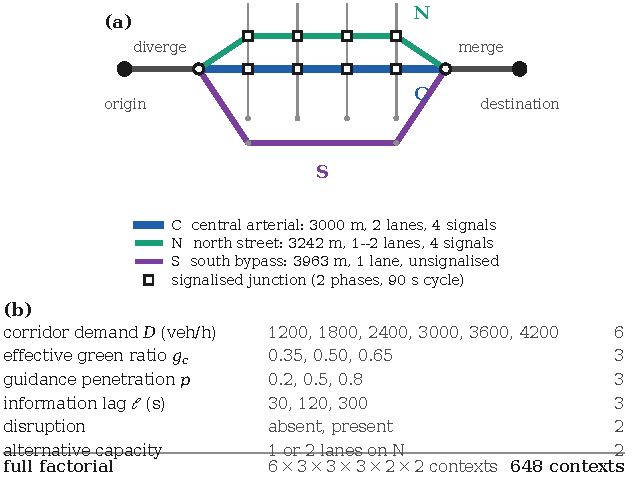
\includegraphics[width=\linewidth]{figures/fig1_network_design.pdf}
\caption{(a) The network. A single origin--destination corridor is served by
three parallel routes between the diverge and the merge: the short signalised
arterial C, the longer signalised street N, and the long unsignalised bypass S.
Cross streets carry fixed background demand. (b) The experimental factors and
their levels. The full factorial gives 648 contexts, each simulated under four
policies with five paired seeds.}
\label{fig:network}
\end{figure}

\subsection{Routing Policies}
\label{sec:method:pol}

All four policies choose one element of the three-path catalogue for one vehicle
at its moment of insertion. Three of them read traffic state, and they read it
from one shared observation buffer, so no policy has an information advantage
over another. The buffer stores the instantaneous travel time of every corridor
edge at a 30\,s sampling interval. A policy acting at time $t$ may read only
samples with timestamp at most $t-\ell$, where $\ell$ is the context's
information lag, and only the most recent 120\,s of those. Before any admissible
sample exists it falls back to free-flow times. No policy sees the future, and
none sees any realised outcome of the run it belongs to. Table~\ref{tab:policies}
states each policy; the parameters were frozen before any evaluation run and are
varied only in the sensitivity experiment of Section~\ref{sec:design:sens}.

\begin{table}[htbp]
\centering\small
\caption{The four routing policies. $L(p)$ is path length; $\hat\mu_p$ and
$\hat\sigma_p$ are the mean and standard deviation of the path travel time over
the visible observation window; $u_e$ is the utilisation of link $e$.}
\label{tab:policies}
\begin{tabularx}{\linewidth}{@{}>{\raggedright\arraybackslash}p{0.085\linewidth}
>{\raggedright\arraybackslash}p{0.30\linewidth}R@{}}
\toprule
& Objective and rule & Information used, parameters, and intended behaviour\\
\midrule
P1 & Shortest distance:
$\arg\min_p L(p)$ &
No traffic state at all. The zero-information reference, and the only policy
whose choice does not vary within a context. It loads the shortest corridor
whether or not that corridor has capacity.\\[2pt]
P2 & Reactive travel time:
$\arg\min_p \hat\mu_p(t-\ell)$ &
Lagged link travel times. Reactive rather than predictive: it extrapolates
nothing, so the estimate it acts on is $\ell$ seconds old. Its hypothesised
failure mode is moving the whole guided cohort together onto a corridor that was
best one lag ago.\\[2pt]
P3 & Capacity-aware load balancing: among paths with
$\hat\mu_p \le (1+\epsilon)\min_q \hat\mu_q$, take
$\arg\min_p \max_{e \in p} u_e$ &
Lagged travel times and flows, plus the policy's own recent assignments that
have not yet cleared a link. Follows the flow-balanced $k$-shortest-path family
\citep{pan2013proactive}. Frozen $\epsilon=0.20$, assignment window 120\,s. It
spreads load when capacity is uneven and wastes time when there is no capacity
shortage.\\[2pt]
P4 & Reliability-aware mean--variance:
$\arg\min_p [\hat\mu_p + \lambda\hat\sigma_p]$ &
Lagged link travel times. $\hat\sigma_p$ is the dispersion of the \emph{path}
travel time across sample instants, so edge correlations within a path are
preserved and the dispersion is observed rather than modelled. Frozen
$\lambda=1.0$. Follows mean--variance route guidance
\citep{sen2001meanvariance}; it avoids volatile corridors and is
over-conservative when variance carries no risk.\\
\bottomrule
\end{tabularx}
\end{table}

Eco-routing is not in the portfolio. It was admitted only conditionally, on the
screening evidence of genuine decoupling between travel time and \CO; that
evidence did not appear (Section~\ref{sec:design:screen}), and the exclusion is
therefore a reported finding rather than a design assumption.

\subsection{Experimental Factors}
\label{sec:method:fac}

Six factors define a context (Fig.~\ref{fig:network}b). Corridor demand takes
six levels from 1200 to 4200\,veh/h, spanning free flow to oversaturation of the
shortest corridor. The effective green ratio takes three levels, which changes
the capacity of both signalised corridors without changing the network. Guidance
penetration takes three levels, which changes the size of the cohort a policy
actually controls, and is the factor most directly implicated in the
herding results of Section~\ref{sec:lit:routing}. Information lag takes three
levels from 30 to 300\,s, which is the staleness of the state a reactive policy
acts on. A disruption regime is present or absent; when present, one lane closure
on the arterial is drawn from a declared distribution --- edge uniform over the
three arterial links, onset uniform on $[600,1200]$\,s, duration uniform over
$\{300,600,900\}$\,s --- from a stream seeded by the run seed alone, so the
realisation is a property of the context and seed and never of the policy.
Alternative capacity is one or two lanes on the north street, which determines
whether load balancing has anything to balance. The full factorial is
$6\times3\times3\times3\times2\times2 = 648$ contexts.

\subsection{Performance Criteria}
\label{sec:method:crit}

Three criteria are recorded for every run. $C_1$ is the mean journey time over
the measured cohort, in seconds per vehicle, and includes insertion delay: a
policy that oversaturates the network produces vehicles that cannot enter it, and
excluding their wait would credit the policy for the queue it caused. $C_2$ is
total tailpipe \CO\ over the cohort. $C_3$ is total stopped delay, the time
vehicles spend below 0.1\,m/s, which is what queueing costs in a form that
neither of the other two isolates.

$C_1$ is the primary decision cost. It is chosen because it requires no weights
and is the quantity a guidance system is usually asked to reduce; using it does
not assert that the other two are unimportant, and Section~\ref{sec:criteria}
reports how often they disagree with it. The three criteria are compared by
Pareto dominance rather than scalarised, and scalarisation appears only as a
declared sensitivity analysis over three normalised preference profiles. No
monetary value of time, value of reliability or carbon price is used, because no
verified source for any of them was available for this setting and inventing one
would make the resulting trade-off an artefact of the assumption.

\subsection{Selector Models}
\label{sec:method:sel}

A selector maps a context to a policy using eight dimensionless descriptors of
the context, listed in Table~\ref{tab:desc}. Each is a function of the context
definition alone; none can be computed from any outcome, and the disruption
descriptor encodes that a disruption \emph{may} occur, never its realisation.
The descriptors are chosen to be mechanistically interpretable rather than
maximally predictive, so that a rule expressed in them has a traffic reading.

\begin{table}[htbp]
\centering\small
\caption{The eight context descriptors. $D$ is corridor demand, $p$ penetration,
$\ell$ information lag, $g$ the effective green ratio, and $\mathrm{cap}_C$,
$\mathrm{cap}_N$, $\mathrm{cap}_S$ the corridor capacities implied by $g$ and the
lane configuration. $T^{\mathrm{ff}}_C$ is the free-flow time on the arterial.}
\label{tab:desc}
\begin{tabularx}{\linewidth}{@{}>{\raggedright\arraybackslash}p{0.10\linewidth}
>{\raggedright\arraybackslash}p{0.30\linewidth}R@{}}
\toprule
& Definition & Reading\\
\midrule
$x_1$ & $D/(\mathrm{cap}_C+\mathrm{cap}_N+\mathrm{cap}_S)$ & network saturation\\
$x_2$ & $D/\mathrm{cap}_C$ & saturation of the shortest corridor if it took all demand\\
$x_3$ & $\mathrm{cap}_N/(\mathrm{cap}_C+\mathrm{cap}_N+\mathrm{cap}_S)$ & share of capacity on the alternative\\
$x_4$ & $(g\,T_{\mathrm{cyc}}-y)/T_{\mathrm{cyc}}$ & effective green ratio\\
$x_5$ & $p$ & guidance penetration\\
$x_6$ & $\ell/T^{\mathrm{ff}}_C$ & information staleness relative to a free-flow trip\\
$x_7$ & disruption indicator & whether a disruption may occur\\
$x_8$ & $p\,D/\mathrm{cap}_C$ & controlled-flow saturation: the share of the shortest corridor's capacity that the guided cohort alone would consume\\
\bottomrule
\end{tabularx}
\end{table}

Five selectors are evaluated on a common footing, together with the two
references of Section~\ref{sec:problem:regret}:

\begin{description}
\item[B0, fixed policy.] The single best fixed policy of Eq.~\eqref{eq:sbs},
identified on the training contexts of each fold. This is the baseline
adaptation must beat, and it is a fitted quantity.
\item[B1, mechanistic rule.] A depth-2 decision tree on the eight descriptors,
fitted to the identity of the per-context winner. It is included because it is
the kind of rule an engineer would write, and because its splits are readable as
traffic statements.
\item[B2, deeper tree.] The same construction at depth 3.
\item[B3, logistic.] Multinomial logistic regression on the standardised
descriptors, again fitted to the winner's identity.
\item[B4, advantage GBDT.] Gradient-boosted regression
\citep{friedman2001gbm,ke2017lightgbm}, but trained on a different target: for
each policy $a$ it predicts the \emph{advantage}
$\Delta_a(s) = C(s,a^{\mathrm{SB}}) - C(s,a)$ over the training-fold fixed
policy, and selects $\arg\max_a \hat\Delta_a$. This is the predict-then-optimise
construction \citep{elmachtoub2022spo}: the model is fitted to decision cost
rather than to the winner's label, so an error that does not change the ordering
costs nothing.
\item[B5, selective.] B4 with two gates. A \emph{support} gate flags a context
whose mean distance to its five nearest training contexts, in the standardised
descriptor space, exceeds the 95th percentile of that statistic within the
training fold. A \emph{confidence} gate requires the split-conformal lower bound
on the predicted advantage, at miscoverage $\alpha=0.10$ calibrated on a held-out
30\,\% of the training fold, to be positive. The selector acts only if both gates
pass; otherwise it abstains to B0. This is a reject option
\citep{chow1970reject} built on split conformal prediction
\citep{vovk2005alrw,lei2018conformal}.
\end{description}

All hyperparameters were fixed in the frozen specification before any evaluation
run and are not tuned. No neural, graph, reinforcement-learning or bandit model
is used: the question is whether a flexible model adds anything over a
transparent rule, not which flexible model wins.

\subsection{Distribution-Shift Framework}
\label{sec:method:shift}

Eight shift splits are evaluated, each declared before the analysis and each
reported on its own. Pooling them would hide the only thing the experiment can
say about them, which is that they behave differently. Splits O1--O6 hold out an
entire level of one factor, so the test marginal of that factor lies outside the
training range; O7 trains without any disruption and tests under disruption, so
both the covariate distribution and the conditional relationship change; O8 is a
separate campaign in which the disruption occurs on the north corridor, which
carries no disruption in any training context. The taxonomy and the training and
test domains are given with the results in Table~\ref{tab:shift}.

For each split the selector, its scales, the fixed-policy baseline, the conformal
quantiles and the support envelope are all refitted on the training side, exactly
as in the main protocol.

\subsection{Statistical Evaluation}
\label{sec:method:stats}

Every context is replicated with five paired seeds under common random numbers:
the vehicle set, departure times, guided and unguided labelling, habitual
corridor choice, background traffic and the disruption realisation are functions
of the seed and the context only, never of the policy. Two runs of a context
under different policies therefore face identical vehicles, and every comparison
between policies is a paired comparison.

An advantage of $a$ over $b$ in context $s$ is called \emph{resolved} when, over
the paired seed differences $d_i = C_1(s,a,i) - C_1(s,b,i)$,
\begin{equation}
|\bar d| \;>\; 2\, \mathrm{sd}(d)/\sqrt{n}.
\label{eq:resolve}
\end{equation}
Eq.~\eqref{eq:resolve} is a descriptive screen and nothing more: it separates
orderings that outrun their own replication scatter from orderings that do not.
It is not an inferential procedure and is not offered as one. Five replications
leave four degrees of freedom in the standard error, the distribution of the
paired differences is not modelled, there is no null hypothesis, and no
adjustment is made for making the comparison 648 times. No hypothesis test appears in this
paper and no claim of statistical significance is made in it. Differences that
fail the criterion are carried through the analysis as ties, and their number is
reported alongside every count that depends on them.

Where the mean of a quantity over contexts is reported, its dispersion is
characterised by the same paired machinery rather than by an interval derived
from an assumed distribution: Section~\ref{sec:value} compares the headroom in
each context against that context's own noise band, and reports how many
contexts carry a headroom larger than it.

A separate convention is needed for ties on the primary criterion, because they
are common. In 50 of 648 contexts two or more policies produce \emph{exactly}
equal system mean journey time, because at low demand or low penetration they
route the guided cohort identically. Winner counts are therefore reported under
a declared, stable tie-break --- portfolio order $\mathrm{P1} \prec \mathrm{P2}
\prec \mathrm{P3} \prec \mathrm{P4}$ --- alongside the count of contexts with a
unique minimum, so that no count depends on an implementation detail of sorting.

\section{Experimental Design and Computational Study}
\label{sec:design}

\subsection{Screening and Study Specification}
\label{sec:design:screen}

The specification --- factors, levels, policies, parameters, criteria, primary
decision cost, resolution criterion, descriptor set, selector ladder,
hyperparameters, shift splits and validity rules --- was frozen and committed
before any evaluation run. Everything reported below follows it, with one
recorded exception described in Section~\ref{sec:integrity}.

Before the main campaign, a 16-context screen with ten seeds per cell (640 runs)
evaluated four pre-declared gates on the primary criterion: that at least three
policies be strictly best somewhere with a resolved margin (G1); that at least
25\,\% of contexts have a non-singleton Pareto set (G2); that policy pairs not be
effectively identical on average (G3); and that no single factor explain the
winner map almost entirely (G4). G2, G3 and G4 passed. G1 failed, with two
policies rather than three.

\subsection{Main Factorial Campaign}
\label{sec:design:main}

The main campaign is the $648 \times 4 \times 5$ design: every context under
every policy at every seed, $12{,}960$ runs. It is the basis of every result in
Sections~\ref{sec:validity}--\ref{sec:criteria} and \ref{sec:selection}.

\subsection{Boundary Refinement}
\label{sec:design:boundary}

The main grid samples demand every 600\,veh/h, so it can locate a change in the
preferred policy only to within a 600\,veh/h bracket. Where the resolved winner
changes between adjacent demand levels, a refinement campaign inserts three
intermediate levels at 150\,veh/h spacing inside that bracket, holding all other
factors fixed. Nineteen such transitions were refined, at 1140 runs. A grid
cannot locate a boundary more finely than its own spacing, so the refined result
is reported as a bracket between adjacent sampled levels and never as a
continuous threshold.

\subsection{Sensitivity Experiments}
\label{sec:design:sens}

Two policy parameters had to be chosen and were frozen: the admissibility
tolerance $\epsilon$ of P3 and the risk weight $\lambda$ of P4. A separate
campaign of 1920 runs re-simulates a 96-context subset at
$\epsilon \in \{0.1, 0.3\}$ and $\lambda \in \{0.5, 1.5\}$ to measure how much
the frozen choice matters. The frozen values are not revised in the light of this
experiment; the result is reported as a property of the benchmark
(Section~\ref{sec:robust}).

A second, purely analytical sensitivity varies the preference profile over the
three criteria across three declared normalised weightings, to test whether the
choice of preferred policy depends on the weights.

\subsection{Distribution-Shift Experiments}
\label{sec:design:shift}

Splits O1--O7 are constructed from the main campaign by holding out factor
levels. O8 required a campaign of its own, because no context in the main
factorial contains a disruption anywhere other than on the arterial: 54 contexts
with a north-corridor disruption, 1080 runs.

\paragraph{A planned split that proved infeasible}
The domain-shift split was originally specified as a disruption on the
\emph{south bypass}, which would have been the strongest available test because
the bypass is the reliability-aware policy's preferred corridor. The
corresponding campaign of 2160 runs was generated and executed, and every one of
the 2160 runs failed. The reason is structural rather than computational: the
bypass is a single-lane corridor, so closing a lane on it does not reduce its
capacity, it disconnects it, and the simulator correctly reported that affected
vehicles had no valid route. A lane closure is a capacity reduction only on a
link with more than one lane. The split was replaced by the north-corridor
disruption reported as O8, which is a genuine domain shift --- no training
context contains a disruption on that corridor --- but is a weaker test than the
one originally planned, because the north corridor is not the corridor that any
policy specialises in. The failed campaign is reported in the ledger, the
replacement is not presented as the original design, and the substitution is
counted as a deviation in Section~\ref{sec:integrity}.

\subsection{Campaign Ledger}
\label{sec:design:ledger}

Table~\ref{tab:ledger} reconciles every simulation executed in the study. The
distinction matters because two different totals are defensible and only one of
them supports the results: $12{,}960$ valid runs constitute the main campaign and
every result in Sections~\ref{sec:validity}--\ref{sec:criteria} derives from
them, while $20{,}284$ simulations were attempted across all campaigns, of which
$18{,}124$ succeeded. Neither number is used where the other is meant.

\begin{table}[htbp]
\centering\footnotesize
\caption{Campaign ledger. Every simulation executed in the study, reconciled.
Completion is the fraction of generated vehicles that reached their destination
within the simulated horizon; a run is valid only at completion $\ge 0.98$ with
no teleports.}
\label{tab:ledger}
\setlength{\tabcolsep}{2.6pt}
\begin{tabular}{@{}llrrrrrr@{}}
\toprule
Campaign & Purpose & Runs & Failed & Contexts & Pol. & Seeds & Compl.\\
\midrule
Screen & complementarity screen & 640 & 0 & 16 & 4 & 10 & 1.000\\
Validate & scenario validation & 384 & 0 & 96 & 4 & 1 & 0.973\\
\textbf{Main} & \textbf{main factorial} & \textbf{12{,}960} & \textbf{0} & \textbf{648} & \textbf{4} & \textbf{5} & \textbf{1.000}\\
Boundary & boundary refinement & 1{,}140 & 0 & 19 brack. & 4 & 5 & 1.000\\
Sensitivity & policy parameters & 1{,}920 & 0 & 96 & 2 & 5 & 1.000\\
O8 north & domain shift & 1{,}080 & 0 & 54 & 4 & 5 & 1.000\\
O8 bypass & domain shift, infeasible & 0 & 2{,}160 & --- & 4 & 5 & ---\\
\midrule
\multicolumn{2}{@{}l}{Attempted} & 20{,}284 & & & & &\\
\multicolumn{2}{@{}l}{Succeeded} & 18{,}124 & & & & &\\
\bottomrule
\end{tabular}
\end{table}

\subsection{Experimental Integrity and Deviations}
\label{sec:integrity}

Two deviations from the frozen specification are recorded, and both are reported
here rather than in a supplement because each changes how a reader should weigh
a result.

\paragraph{D-1: the screening gate failed and the campaign was run anyway}
The frozen rule stated that if G1, G3 or G4 failed, the main campaign would not
be run and the study would report a negative result about portfolio design. G1
failed: only two policies, P1 and P3, were strictly best somewhere with a
resolved margin, against a threshold of three. The main campaign was run
regardless. This is a protocol deviation and is not resolved by reinterpreting
the rule.

The reasons were recorded before the campaign was launched and none of them is a
result the campaign might produce. First, the gate's purpose was satisfied: it
exists to prevent a selection study being built on a portfolio with no selection
problem, and a selection problem demonstrably existed, with the preferred policy
reversing between P1 and P3 at resolved margins up to 18.0\,\%. Second, the gate
was written against the primary criterion alone and was blind to the
multi-criteria structure beside it: G2 passed, and all four policies appeared in
Pareto sets, the reliability-aware policy most often of all. Third, the negative
finding was not yet supportable: the screen sampled 16 contexts at extreme factor
levels only and never sampled the demand transition region, so stopping would
have asserted a negative from a small and badly placed fraction of the design.

Four constraints were declared at the same time, before the campaign: that the
study may not claim four-way complementarity on the primary criterion; that it
may not claim P2 or P4 is ever the best journey-time policy unless the full
campaign resolves such a win; that G1's failure must be reported as a finding;
and that a confirmatory gate G1$'$ --- the identical definition evaluated on all
648 contexts --- be declared in advance and its result reported whichever way it
came out. Section~\ref{sec:complementarity} reports that result.

The methodological lesson is recorded as such, because it generalises beyond this
study: a complementarity screen must cover the interior of the factor space and
not only its corners. A resolution-IV fraction at extreme levels is an efficient
design for estimating main effects and a poor one for discovering where a winner
map changes. A gate that is passed only after being overridden was a badly
designed gate.

\paragraph{D-2: the domain-shift split was replaced}
The originally specified O8 was infeasible for the structural reason given in
Section~\ref{sec:design:shift}, and was replaced by a weaker but valid
alternative. The replacement is labelled as such wherever it appears.

\section{Results}
\label{sec:results}

\subsection{Campaign Validity}
\label{sec:validity}

All $12{,}960$ runs of the main campaign completed. Completion is 1.0000 in
every run, minimum and mean alike, and the total teleport count is zero, so no
run was discarded and no context was excluded: all 648 are analysed, each with
four policies at five seeds. The campaign contains approximately 22.0 million
simulated vehicle trips. Because validity is exact rather than near-exact, none
of the results below involves a selection decision about which runs to keep.

\subsection{Policy Complementarity}
\label{sec:complementarity}

\paragraph{The confirmatory gate}
Gate G1$'$, declared before the campaign and evaluated on all 648 contexts,
\textbf{passes}: three policies --- P1, P3 and P4 --- are strictly best in at
least one context with a resolved margin, against the threshold of three. The
resolved winner counts are P3 227, P4 19 and P1 11, with 257 of 648 contexts
resolved. \textbf{P2 is never a resolved winner}, which confirms on the full
factor space what the screen saw in its 16 contexts. The screen's STOP verdict
was therefore a sampling artefact of the screening design rather than a property
of the portfolio: the screen had the power to detect near-ties, which it did
correctly, but not the coverage to find the regions where P1 and P4 win.

\paragraph{Ties are common and are reported as such}
In 50 of 648 contexts (7.7\,\%) two or more policies produce exactly equal system
mean journey time, because at low demand or low penetration they route the guided
cohort identically. The tied sets are P2 with P4 in 39 contexts, P2 with P3 and
P4 in 8, and P3 with P4 in 3. Under the declared tie-break the winner counts are
P3 418, P4 129, P2 80 and P1 21; restricting to the 598 contexts with a unique
minimum gives P3 415, P4 129, P2 33 and P1 21. We report both, because a count
that changes by 47 contexts depending on how ties are broken should not be
presented as a single number.

\paragraph{Most differences do not survive replication}
Of the 648 contexts, 391 (60.3\,\%) have an unresolved winning margin. Those
margins are negligible rather than merely uncertain: their median is 0.13\,\% of
the best journey time, against a median of 5.20\,\% among resolved margins, which
reach 26.9\,\% (Fig.~\ref{fig:comp}b). With five paired seeds under common random
numbers a 5\,\% difference resolves comfortably, so the unresolved cases are
genuine equivalence and not a power failure. The portfolio is complementary, but
in most contexts the choice among its members does not matter on journey time.

\paragraph{Two policies are largely interchangeable}
Applying the study's operational-identity criterion --- an unresolved paired
difference together with a route split differing by less than 2\,\% of the guided
cohort --- P2 and P4 are indistinguishable in 42.6\,\% of contexts, P2 and P3 in
22.7\,\%, and P3 and P4 in 20.2\,\%. P1 is never indistinguishable from any other
policy, which is expected: it is the only policy that ignores traffic state.
Averaged over the six pairs the identity rate is 14.2\,\%. A nominal portfolio of
four policies therefore behaves, over much of the context space, like a portfolio
of two or three.

\paragraph{The winner map is multi-factor but shallow}
Fig.~\ref{fig:comp}a shows the modal winner over the demand-by-penetration
plane. Predicting the winner with a constant is correct in 64.5\,\% of contexts;
the best single factor, demand, reaches 66.5\,\%; the best pair, demand with
penetration, reaches 70.7\,\%; the best triple, demand with green ratio and
penetration, reaches 79.2\,\%; and all six factors together identify the winner
in every context by construction. The structure is genuinely multi-factor --- no
single factor comes close --- but it is also shallow, in the sense that the
marginal return to context information falls off quickly after the first two
factors. This is the first indication that the decision problem, although real,
is not large.

\begin{table}[htbp]
\centering\scriptsize
\caption{Complementarity of the portfolio over 648 contexts on the primary
criterion, and over all three criteria jointly. ``Best'' uses the declared
portfolio-order tie-break; ``unique best'' counts only the 598 contexts with a
unique minimum; ``resolved best'' requires the margin over the runner-up to
exceed twice its paired standard error.}
\label{tab:comp}
\setlength{\tabcolsep}{3.4pt}
\begin{tabular}{@{}lrrrrr@{}}
\toprule
& P1 & P2 & P3 & P4 & total\\
\midrule
Best on journey time & 21 & 80 & 418 & 129 & 648\\
\quad of which unique best & 21 & 33 & 415 & 129 & 598\\
\quad of which resolved best & 11 & \textbf{0} & 227 & 19 & 257\\
Best on \CO & 10 & 57 & 453 & 128 & 648\\
Best on stopped delay & 0 & 80 & 139 & \textbf{429} & 648\\
In the three-criterion Pareto set & 21 & 266 & 555 & 525 & ---\\
\midrule
\multicolumn{6}{@{}l}{\emph{Operationally indistinguishable pairs} (share of 648 contexts)}\\
\multicolumn{6}{@{}l}{\quad P2--P4 42.6\,\%; \ P2--P3 22.7\,\%; \ P3--P4 20.2\,\%; \ P1 with any other 0.0\,\%}\\
\midrule
\multicolumn{6}{@{}l}{\emph{Winner-map classification rate}}\\
\multicolumn{6}{@{}l}{\quad constant 64.5\,\%; \ best single (demand) 66.5\,\%; \ best pair (demand, penetr.) 70.7\,\%}\\
\multicolumn{6}{@{}l}{\quad best triple (demand, green, penetr.) 79.2\,\%; \ all six factors 100\,\%}\\
\bottomrule
\end{tabular}
\end{table}

\begin{figure}[htbp]
\centering
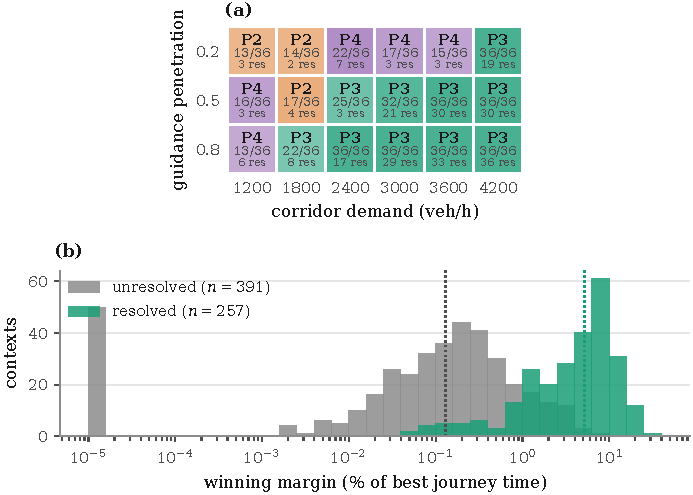
\includegraphics[width=\linewidth]{figures/fig2_complementarity.pdf}
\caption{(a) Modal winning policy over the demand-by-penetration plane, each
cell aggregating 36 contexts; the fraction is the modal winner's share of those
contexts and ``res'' counts contexts whose winning margin is resolved against
replication noise. (b) Distribution of the winning margin, as a percentage of the
best journey time in that context, separated into resolved and unresolved
contexts. Dotted lines mark the two medians. The axis is logarithmic and exact
ties are shown at the left edge.}
\label{fig:comp}
\end{figure}

\subsection{Mechanisms and Preference Boundaries}
\label{sec:mechanism}

The winner map has a physical reading. Fig.~\ref{fig:cost} shows why the
portfolio separates at all: the distance-minimising policy P1 diverges from the
other three as demand rises, because it concentrates the guided cohort on the
arterial regardless of whether the arterial can carry it, while the three
traffic-aware policies remain within a few per cent of each other throughout.
The same figure shows the penetration effect that Section~\ref{sec:lit:routing}
would predict: mean journey time under the traffic-aware policies falls from
penetration 0.2 to 0.5 and then rises again at 0.8, while P1 deteriorates
monotonically. More guidance is not monotonically better, consistent with
\citet{yang1998penetration} and with the concentration mechanism reported by
\citet{cornacchia2026concentration}, although this study does not isolate that
mechanism and the agreement is a consistency check rather than a replication.

\begin{figure}[htbp]
\centering
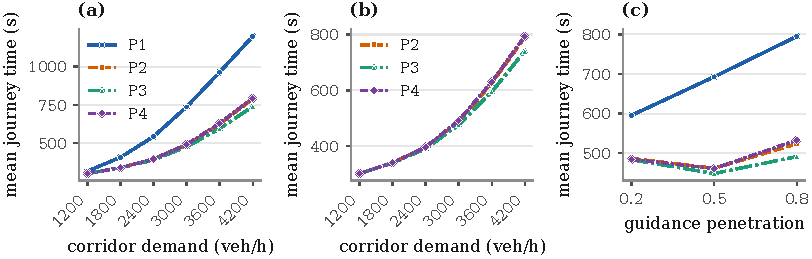
\includegraphics[width=\linewidth]{figures/fig3_cost_landscape.pdf}
\caption{System mean journey time against (a, b) corridor demand and (c)
guidance penetration, averaged over all other factors. Panel (b) repeats panel
(a) without P1 so that the three traffic-aware policies can be distinguished.
Colours and markers are consistent across panels.}
\label{fig:cost}
\end{figure}

Fitting the depth-2 mechanistic rule to the winner's identity on all 648
contexts, for exposition, gives a first split on $x_8 = pD/\mathrm{cap}_C$, the
share of the shortest corridor's capacity that the guided cohort alone would
consume, at a threshold bracketed between the adjacent sampled values 0.748 and
0.781. Below that threshold the rule separates on the effective green ratio;
above it, on whether total demand exceeds arterial capacity. Fig.~\ref{fig:mech}
shows the corresponding structure directly: below $x_8 \approx 0.76$ the
reliability-aware and reactive policies win a substantial share of contexts, and
above it the load-balancing policy wins almost everywhere.

The reading is that the controlling quantity is not demand and not penetration
separately but their product relative to the capacity of the corridor that every
policy would otherwise prefer. When the guided cohort alone would saturate the
arterial, spreading it across corridors is worth doing; when it would not,
spreading it costs more than it saves. That is a statement about association
within a designed factorial. The experiment varies the factors but does not
isolate the mechanism --- it contains no treatment that changes $x_8$ while
holding the physical routes constant --- so no causal claim is made, and the rule
is reported as consistent with the data rather than as identified by it.

\begin{figure}[htbp]
\centering
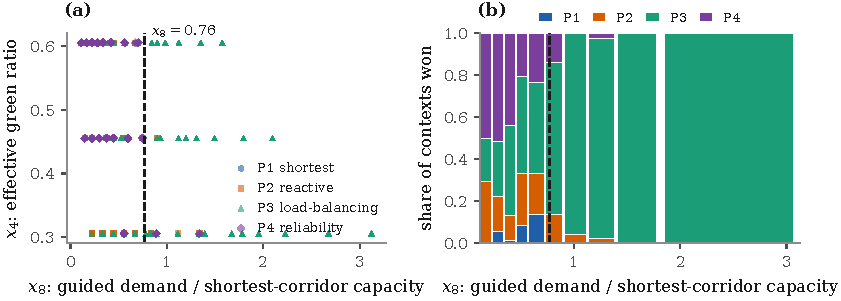
\includegraphics[width=\linewidth]{figures/fig4_mechanism.pdf}
\caption{(a) Contexts in the plane of controlled-flow saturation $x_8$ and
effective green ratio $x_4$, coloured by the winning policy; the dashed line is
the first split of the depth-2 rule fitted to all contexts. (b) Share of
contexts won by each policy in deciles of $x_8$. The transition is a property of
$x_8$ rather than of demand or penetration separately.}
\label{fig:mech}
\end{figure}

\paragraph{Refining the boundary}
Nineteen demand transitions were refined from a 600\,veh/h grid to a 150\,veh/h
grid. Thirteen of them have a single changepoint on the refined grid, and for
nine of those the point-estimate bracket narrows to 150\,veh/h; the remaining
four stay at 600. The other six transitions are \emph{not} monotone in demand:
the winner changes two to five times across the refined sequence. Moreover, of
the thirteen single-changepoint transitions, only seven have either endpoint of
the changepoint interval resolved against replication noise. The honest summary
is that refinement narrows a point estimate but does not deliver a resolved
boundary: a grid cannot locate a boundary more finely than its own spacing, and
at this spacing the winner sequence is, in a third of cases, not even monotone.
No continuous threshold is reported anywhere in this paper.

\subsection{Decision Value}
\label{sec:value}

This is the central result. The single best fixed policy over all 648 contexts is
P3, with a system mean journey time of 474.35\,s per vehicle. The hindsight best
achieves 473.90\,s. The decision headroom is therefore
\begin{equation}
H = 474.35 - 473.90 = 0.45\ \text{s per vehicle},
\end{equation}
which is 0.095\,\% of the fixed policy's own mean cost. Averaging the per-context
ratio instead gives 0.120\,\%; the two are different statistics and the
aggregate is used throughout, with its denominator stated.

Against that, the cost of choosing the wrong fixed policy is large.
Table~\ref{tab:value} gives the penalties: committing to P1 for the whole
benchmark costs 220.21\,s per vehicle more than committing to P3, which is
46.4\,\% of P3's mean cost. P2 and P4 cost 16.34\,s (3.4\,\%) and 18.34\,s
(3.9\,\%). The ratio between the first-order decision --- which fixed policy ---
and the second-order decision --- whether to adapt it --- is roughly 490 to 1.
Fig.~\ref{fig:value}a places the two on the same axis, which requires a
logarithmic scale.

\begin{table}[htbp]
\centering\small
\caption{Decision value on the primary criterion over 648 contexts. Penalty is
the mean cost above the single best fixed policy; headroom is the mean cost of
the single best fixed policy above the per-context best.}
\label{tab:value}
\begin{tabular}{@{}lrrr@{}}
\toprule
Choice & Mean journey & Penalty & Penalty\\
 & time (s/veh) & (s/veh) & (\%)\\
\midrule
Fix P1 (shortest) & 694.56 & 220.21 & 46.42\\
Fix P4 (reliability) & 492.69 & 18.34 & 3.87\\
Fix P2 (reactive) & 490.69 & 16.34 & 3.44\\
Fix P3 (load balancing, SBS) & 474.35 & 0.00 & ---\\
\midrule
Hindsight best (VBS) & 473.90 & $-0.45$ & $-0.095$\\
\bottomrule
\end{tabular}
\end{table}

\paragraph{Why the headroom is so small}
The fixed policy is near-dominant rather than merely good. P3 attains the
per-context minimum in 426 of 648 contexts (65.7\,\%). In the 222 contexts where
it does not, it loses on average 1.32\,s and at worst 17.19\,s. In the contexts
where it does win, it wins by 22.47\,s on average. The upside of the fixed policy
is therefore about 17 times its downside, and an adaptive layer competes only
for the downside. A portfolio can be complementary in the sense of
Section~\ref{sec:complementarity} while this ratio makes adaptation nearly
worthless, and that is what happens here.

\paragraph{Most of the headroom is not resolvable}
The headroom must also be compared against the replication noise of the
experiment that measured it. Fig.~\ref{fig:value}c plots, for each of the 222
contexts where the fixed policy is not best, the headroom in that context against
that context's own $2\,$SE band on the paired difference. Only 55 of the 222
(24.8\,\%) carry a headroom larger than their own noise band. The mean noise band
in those contexts is 1.67\,s, against a mean headroom of 1.32\,s. Resolving the
campaign-wide mean effect of 0.45\,s at the same criterion would require
approximately 25 seeds per context rather than five, that is about 64{,}800 runs
instead of 12{,}960. This is stated as a property of the effect size, not as a
recommendation: an effect that needs 25 replications per cell to separate from
simulation noise is unlikely to be the deciding consideration in a deployment.

\begin{figure}[htbp]
\centering
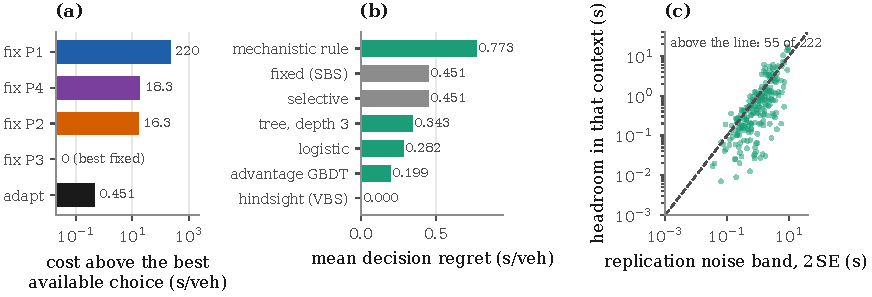
\includegraphics[width=\linewidth]{figures/fig5_decision_value.pdf}
\caption{(a) Cost of each available commitment above the best one, on a
logarithmic axis: the penalty for the wrong fixed policy dwarfs the headroom
available to adaptation. (b) Mean decision regret of every rule under
leave-one-context-out evaluation. (c) For each of the 222 contexts where the
fixed policy is not the per-context best, the headroom in that context against
its own replication noise band; points above the dashed line are contexts whose
headroom exceeds the dispersion of the experiment that measured it.}
\label{fig:value}
\end{figure}

\subsection{Selector Comparison}
\label{sec:selection}

Table~\ref{tab:ladder} reports every rule under identical leave-one-context-out
evaluation, in which the model, its scales, the fixed-policy baseline, the
conformal quantiles and the support envelope are all refitted from the 647
training contexts of each fold, and all five replications of the held-out context
move together. Two findings matter more than the ordering itself.

\begin{table}[htbp]
\centering\footnotesize
\caption{Selector ladder under leave-one-context-out evaluation on 648 contexts.
Regret is in seconds per vehicle. ``Gap closed'' is $G(\pi)$ of
Eq.~\eqref{eq:headroom}: the share of the fixed policy's headroom recovered.
``Top-1'' is the fraction of contexts in which the chosen policy is the observed
best, and is reported to be contrasted with regret, not to rank the rules.}
\label{tab:ladder}
\setlength{\tabcolsep}{3.0pt}
\begin{tabular}{@{}llrrrrrr@{}}
\toprule
& Rule & Mean & Median & Max & CVaR$_{90}$ & Top-1 & Gap closed\\
\midrule
B1 & mechanistic rule & 0.773 & 0.000 & 17.19 & 6.47 & 66.7\,\% & $-71.4$\,\%\\
B0 & fixed policy (SBS) & 0.451 & 0.000 & 17.19 & 3.67 & 64.5\,\% & 0.0\,\%\\
B5 & selective (gated B4) & 0.451 & 0.000 & 17.19 & 3.67 & 64.5\,\% & 0.0\,\%\\
B2 & tree, depth 3 & 0.343 & 0.000 & 17.19 & 3.02 & 73.9\,\% & $+23.8$\,\%\\
B3 & logistic & 0.282 & 0.000 & 17.19 & 2.55 & \textbf{76.1}\,\% & $+37.4$\,\%\\
B4 & advantage GBDT & \textbf{0.199} & 0.000 & \textbf{6.96} & \textbf{1.66} & 73.1\,\% & $\mathbf{+55.8}$\,\%\\
\midrule
& hindsight best (VBS) & 0.000 & 0.000 & 0.00 & 0.00 & 100\,\% & $+100$\,\%\\
\bottomrule
\end{tabular}
\end{table}

\paragraph{The mechanistic rule is more accurate and more expensive than doing
nothing.} B1 identifies the winning policy in 66.7\,\% of contexts against the
fixed policy's 64.5\,\%, and yet its mean regret is 0.773\,s against 0.451\,s ---
it closes $-71$\,\% of the headroom, which is to say it opens a gap of its own.
The explanation is visible in the tail: B1 and B0 share the same worst case, but
B1's CVaR$_{90}$ is 6.47\,s against 3.67\,s. The rule deviates from the fixed
policy in contexts where it is right about the ordering and wrong about the
magnitude, gaining a fraction of a second when correct and losing several seconds
when not. Selecting the right policy more often is not the same as deciding
better, and a study that reported accuracy alone would have concluded that the
mechanistic rule works.

\paragraph{Training on decision cost changes the ordering} B3, the most accurate
rule at 76.1\,\%, is not the cheapest. B4 is less accurate at 73.1\,\% and
recovers substantially more headroom, 55.8\,\% against 37.4\,\%, because it is the
only rule fitted to advantage rather than to the winner's identity: it learns how
much a policy is worth rather than which policy wins, so it deviates from the
fixed policy only where the predicted gain is large. The consequence appears in
the tail statistics, which are the ones an operator would care about. B4 is the
only rule that reduces the worst case, from 17.19\,s to 6.96\,s, and it more than
halves CVaR$_{90}$, from 3.67\,s to 1.66\,s. It deviates from the fixed policy in
233 of 648 contexts and leaves the fixed policy in place in the rest. This is the
predict-then-optimise distinction \citep{elmachtoub2022spo} appearing in a traffic
setting, and it is the one place in this study where the choice of learning target
--- not the choice of model class --- changes the answer.

\paragraph{What the gain is worth} Closing 55.8\,\% of the headroom means
reducing mean journey time from 474.35\,s to 474.10\,s, a saving of 0.25\,s per
vehicle, or 0.053\,\%. The selector works, in the sense that it does what it was
asked to do on held-out contexts, and it is not worth deploying for that gain.
Both halves of that sentence are results.

\subsection{Multi-Criteria Structure}
\label{sec:criteria}

Complementarity looks quite different on the criterion vector than on the scalar.
Over the three criteria jointly, 473 of 648 contexts (73.0\,\%) have more than one
non-dominated policy, and the mean Pareto set contains 2.11 of the four policies
(Fig.~\ref{fig:crit}a). Pareto membership is P3 in 555 contexts, P4 in 525, P2 in
266 and P1 in 21.

The reliability-aware policy is the clearest case of criterion specialisation.
P4 minimises total stopped delay in 429 of 648 contexts, more than any other
policy, while minimising journey time in only 129 and \CO\ in 128
(Fig.~\ref{fig:crit}b). It achieves this by routing to the steady unsignalised
bypass: vehicles spend longer in the network but less of that time stationary.
A study that ranked policies on journey time alone would record P4 as a marginal
member of the portfolio; on stopped delay it is the leading one. The
distance-minimising policy P1 is the opposite case --- it never minimises stopped
delay in any context.

\begin{figure}[htbp]
\centering
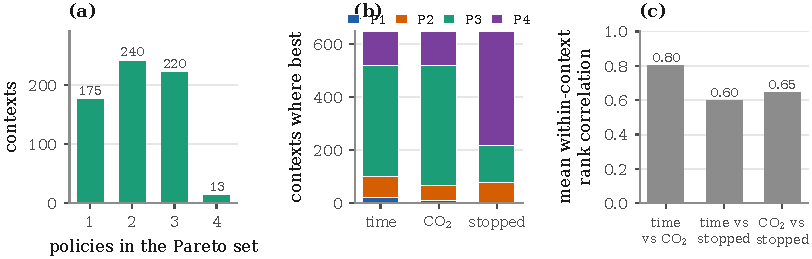
\includegraphics[width=\linewidth]{figures/fig6_criteria.pdf}
\caption{(a) Number of non-dominated policies per context over journey time,
\CO\ and stopped delay. (b) Which policy minimises each criterion, counted over
the 648 contexts. (c) Mean within-context Spearman correlation between criteria
across the four policies, which is the correlation that governs whether the
criteria order policies the same way.}
\label{fig:crit}
\end{figure}

The criteria are correlated but not interchangeable. Pooled across all
context--policy cells the Pearson correlations are 0.94 for journey time against
\CO, 0.89 against stopped delay and 0.89 between \CO\ and stopped delay; but the
quantity that matters for a decision is the within-context correlation across the
four policies, and that is 0.80, 0.60 and 0.65 respectively
(Fig.~\ref{fig:crit}c). The best policy on \CO\ differs from the best on journey
time in 192 contexts (29.6\,\%), and the best on stopped delay differs in 363
(56.0\,\%).

Two consequences follow. First, stopped delay carries decision information that
journey time and \CO\ do not, and it is the criterion on which the portfolio is
most complementary. Second, the close alignment of journey time and \CO\ is the
evidence that led to eco-routing being excluded from the portfolio: with a
within-context rank correlation of 0.80 and identical policy orderings in
52.2\,\% of contexts, a standalone environmental objective has little room to
differ from a time-based one in this network. That exclusion is therefore a
finding about this environment, not an assumption, and it should not be read as a
general statement about eco-routing.

Crucially, a large Pareto set is not evidence that adaptation is valuable. A set
can be large because the criteria disagree about an ordering while all the
differences are small. That is what happens here: 73.0\,\% of contexts have more
than one non-dominated policy, and the decision value on the primary criterion is
0.45\,s per vehicle. Complementarity on the criterion vector and decision value on
the decision criterion are different quantities, and this benchmark separates them
by two orders of magnitude.

\subsection{Distribution Shift}
\label{sec:shift}

Table~\ref{tab:shift} reports the eight splits separately. Pooling them would
produce an average that describes none of them.

\begin{table}[htbp]
\centering\scriptsize
\setlength{\tabcolsep}{3.2pt}
\caption{Distribution shift, by type. Regret is mean decision regret in seconds
per vehicle on the held-out contexts. ``Flagged'' is the share of held-out
contexts the support gate declared outside the training envelope; ``abstained''
is the share on which the selective rule declined to act. A split is classified
as helping or harming when the selector's regret differs from the fixed policy's
by more than the declared 0.05\,s tolerance.}
\label{tab:shift}
\begin{tabular}{@{}llrrrrrrl@{}}
\toprule
Split & Shift type & Tr. & Te. & Fixed & GBDT & Selec. & Flag. & Verdict\\
\midrule
O3 demand $=2400$ & interpolation (control) & 540 & 108 & 0.565 & 0.167 & 0.565 & 0\,\% & helps\\
O2 demand $=1200$ & extrapolation, below & 540 & 108 & 0.528 & 0.531 & 0.528 & 15\,\% & neutral\\
O1 demand $=4200$ & extrapolation, above & 540 & 108 & 0.000 & 0.983 & 0.000 & 43\,\% & \textbf{harms}\\
O4 lag $=300$\,s & extrapolation, above & 432 & 216 & 0.232 & 0.237 & 0.232 & 100\,\% & neutral\\
O5 penetration $=0.8$ & extrapolation, above & 432 & 216 & 0.298 & 0.293 & 0.298 & 100\,\% & neutral\\
O6 green $=0.65$ & extrapolation, above & 432 & 216 & 1.040 & 1.157 & 1.040 & 100\,\% & \textbf{harms}\\
O7 disruption present & covariate $+$ concept & 324 & 324 & 0.630 & 2.216 & 0.630 & 32\,\% & \textbf{harms}\\
O8 north disruption & domain shift & 648 & 54 & 0.314 & 0.176 & 0.314 & \textbf{0\,\%} & helps\\
\bottomrule
\end{tabular}
\end{table}

At the declared tolerance the unguarded selector \textbf{helps on two} splits
(the interpolation control O3 and the domain shift O8), is
\textbf{indistinguishable on three} (O2, O4, O5) and \textbf{harms on three}
(O1, O6 and, worst, the concept shift O7). It is not the case that the selector
degrades under every shift, and it is not the case that shift is harmless; the
behaviour depends on the shift, which is why the splits are not pooled.

Three observations carry most of the content.

\paragraph{The worst failure is the concept shift} O7 trains without any
disruption and tests under disruption, so both the covariate distribution and the
conditional relationship between context and policy performance change. The fixed
policy incurs 0.630\,s of regret there; the selector incurs 2.216\,s, more than
three times as much. Extrapolating a factor level is survivable in this benchmark;
learning a relationship that no longer holds is not.

\paragraph{Extrapolation above the training range is where the selector does
damage.} O1 holds out the highest demand. There the fixed policy is optimal in
every one of the 108 held-out contexts, so its regret is exactly zero, and any
deviation is pure loss: the selector incurs 0.983\,s. A tree-based regressor
cannot extrapolate --- beyond the largest training value of a feature it returns
the prediction of its outermost leaf --- and here that leaf was fitted where the
fixed policy was not always best.

\paragraph{The support gate does not detect the shift it was built for} The gate
flags 100\,\% of held-out contexts on the three extrapolation splits O4, O5 and
O6, which is the behaviour it was designed for. It flags 43\,\% on O1 and 32\,\%
on O7. It flags \textbf{none} of the 54 held-out contexts of O8
(Fig.~\ref{fig:shift}b), despite O8 being the only genuine domain shift in the
set. The reason is not a tuning failure but a representation failure: the
descriptor $x_7$ encodes that a disruption may occur, not where it occurs, so a
disruption relocated to a different corridor is invisible in the feature space the
gate operates in. A detector that measures distance in a feature space cannot
detect a change that the feature space does not encode. This is a general
limitation of support-based out-of-distribution detection, and it is exactly the
case in which such a gate would be most relied upon. No claim of out-of-
distribution safety is made anywhere in this paper.

\begin{figure}[htbp]
\centering
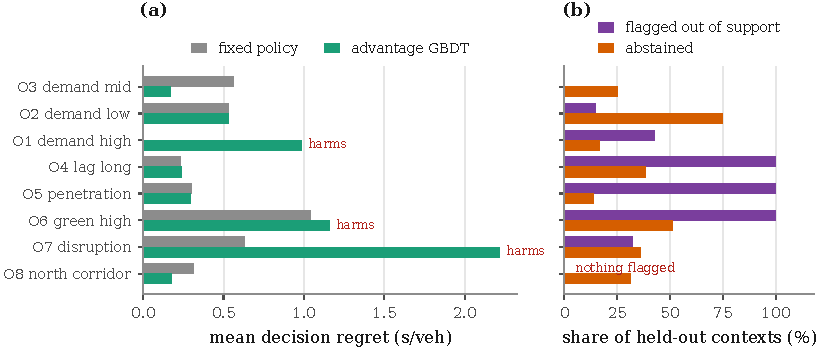
\includegraphics[width=\linewidth]{figures/fig7_shift.pdf}
\caption{(a) Mean decision regret of the fixed policy and the advantage GBDT on
each held-out split. (b) Share of held-out contexts flagged outside the training
support and share on which the selective rule abstained. The support gate flags
every context of the three factor-level extrapolations and none of the domain
shift O8.}
\label{fig:shift}
\end{figure}

\subsection{Selective Prediction}
\label{sec:selective}

The selective rule B5 acts only when the context is inside the support envelope
and the split-conformal lower bound on the predicted advantage is positive.
Its behaviour in this study is unambiguous and entirely negative:

\begin{quote}
B5 chose the fixed policy in \emph{every one} of the 648 contexts, and on
\emph{every one} of the eight shift splits. It abstained in exactly the 233
contexts in which the unguarded selector would have deviated, and in the
remaining 415 the unguarded selector chose the fixed policy anyway. The
confidence gate never certified a single deviation.
\end{quote}

This is not a tuning failure, and it is not a property of the particular
conformal construction. It follows from a ratio. The mean replication noise
floor across contexts --- the largest paired $2\,$SE against the best policy ---
is 20.90\,s per vehicle. The mean advantage available to any deviation is
0.45\,s. A conformal interval calibrated to residuals of that magnitude is
necessarily far wider than the effect it is being asked to certify, so the lower
bound on a predicted advantage is essentially never positive. Any confidence-gated
selector, conformal or otherwise, faces the same arithmetic in this regime.

The consequence is a design rule that generalises beyond this study, and it is
the reverse of the usual framing. Selective prediction is normally presented as
insurance: give up a little in-distribution performance to avoid
out-of-distribution harm. Here the insurance costs everything and pays nothing,
because the premium --- the entire 55.8\,\% of headroom that B4 recovers --- is
larger than the loss being insured against in every split where the selector helps,
and the gate cannot distinguish the splits where it harms. Before building an
abstention mechanism, the effect size should be compared against the replication
noise of the system it will act on; if the ratio is of the order seen here, no
confidence gate can act.

\subsection{Sensitivity and Robustness}
\label{sec:robust}

\paragraph{Policy parameters} Two parameters had to be chosen and were frozen:
the admissibility tolerance $\epsilon$ of P3 and the risk weight $\lambda$ of P4.
Re-simulating a 96-context subset shows that the choice matters, and in one case
matters a great deal. Loosening P3's tolerance from the frozen $\epsilon=0.20$ to
$0.30$ improves its mean journey time by 16.66\,s per vehicle; tightening it to
$0.10$ costs 8.10\,s. Changing P4's $\lambda$ from 1.0 to 0.5 or 1.5 changes its
mean cost by $-0.11$\,s and $+1.27$\,s, with a median change of exactly zero in
both cases, so P4 is insensitive to its parameter over this range while P3 is not.

The frozen values are not revised, and the main analysis is not recomputed at the
better value: doing so after seeing the result would replace a pre-declared
benchmark with a tuned one. The correct reading is that the benchmark is
\emph{conservative} with respect to P3 and that parameter tuning within a single
policy is worth roughly 37 times more on this benchmark than selecting among
policies. That comparison is arguably the most practically useful number in the
study, and it was produced by a robustness check rather than by the main
experiment.

\paragraph{Preference weights} Scoring the three criteria under three declared
normalised profiles changes the preferred policy in 14.5\,\% of contexts. The
time-weighted profile agrees with the primary criterion in 92.9\,\% of contexts,
the balanced profile in 86.0\,\% and the environment-weighted profile in 80.1\,\%.
The decision is therefore not inert with respect to the preference model --- in
contrast to what a strongly aligned criterion set would produce --- but neither is
it dominated by it.

\paragraph{Model capacity} The ladder of Table~\ref{tab:ladder} is itself the
capacity sensitivity: depth-2 tree, depth-3 tree, logistic regression and
gradient boosting span a wide range of flexibility, and the ordering by regret
does not follow the ordering by capacity. The best rule by regret is not the best
by accuracy, and the simplest rule is worse than no rule at all.

\section{Discussion}
\label{sec:discussion}

\subsection{What the Experiment Establishes}
\label{sec:disc:what}

Three things are established on this benchmark, and they should be stated with
their scope attached. First, the portfolio is complementary: three of four
policies are strictly best somewhere with a margin that survives replication, and
73.0\,\% of contexts have more than one non-dominated policy on the criterion
vector. Second, the decision value of that complementarity is 0.45\,s per vehicle
on a 474.4\,s mean, against 220.2\,s for the first-order choice of which fixed
policy to adopt. Third, a selector trained on decision cost recovers 55.8\,\% of
the headroom on held-out contexts and reduces the worst case by more than half,
while remaining worth 0.25\,s per vehicle.

What is \emph{not} established is anything about a real network. One synthetic
three-corridor topology, one origin--destination structure, one signal plan
family and one demand profile were studied. The numbers above are properties of
that benchmark.

\subsection{Why Complementarity Does Not Imply Decision Value}
\label{sec:disc:gap}

The gap between the second and third paragraphs above is the paper's main point,
and it has a mechanism rather than being an accident of this environment.

Complementarity is a statement about the \emph{argmin} of a cost function over a
portfolio; decision value is a statement about the \emph{gap} between the best
fixed member and that argmin. The two coincide only when the best fixed policy is
badly wrong where it is wrong. Here it is not: P3 attains the minimum in two
thirds of contexts, and in the third where it does not it loses 1.32\,s on average
while winning by 22.47\,s where it does. An upside-to-downside ratio of 17 means
the fixed policy absorbs most of the variation in the winner map, leaving
adaptation to compete for a residue.

This has a practical reading that is easy to miss. The right question to ask of a
portfolio is not ``do different members win in different instances?'' --- in any
non-degenerate portfolio some will --- but ``how much does the best fixed member
lose where it loses, and how often?'' Those two quantities, not the count of
distinct winners, determine whether per-instance selection is worth building.
They are cheap to compute from the same data that establishes complementarity,
and reporting only the first while implying the second overstates the case for
adaptation.

The multi-criteria result reinforces the same point from the other side. On the
criterion vector the portfolio looks strongly complementary --- 73.0\,\% of
contexts admit more than one non-dominated policy, and the reliability-aware
policy is the best stopped-delay policy in two thirds of contexts while almost
never being the best journey-time policy. None of that changes the decision value
on the decision criterion. A Pareto set can be large because criteria disagree
about an ordering while every difference is small.

\subsection{Mechanistic Reading of the Boundary}
\label{sec:disc:mech}

Where the preferred policy does change, the organising quantity is the product of
demand and penetration relative to the capacity of the corridor every policy would
otherwise prefer. Below a controlled-flow saturation of roughly 0.76 the guided
cohort is small enough, or the arterial large enough, that diverting traffic costs
more than the congestion it avoids, and the reliability-aware and reactive
policies hold much of the space. Above it the arterial cannot absorb the guided
cohort and load balancing wins almost everywhere. The quantity is dimensionless
and computable before any vehicle departs, which is what makes it usable as a
switching criterion.

Three qualifications belong with that reading. The threshold is a bracket between
adjacent sampled levels, not a number: a grid cannot locate a boundary more finely
than its own spacing, and the refinement campaign showed that at 150\,veh/h
spacing a third of the transitions are not even monotone in demand. The rule is an
association within a designed factorial; the experiment contains no treatment that
manipulates $x_8$ while holding the physical routes fixed, so it does not identify
a mechanism. And the same rule, evaluated as a decision rule rather than as a
description, is worse than doing nothing --- which is the subject of the next
subsection.

\subsection{Why Decision-Oriented Evaluation Changes the Answer}
\label{sec:disc:decision}

The mechanistic rule is more accurate than the fixed policy and costs more than
it. The most accurate learned rule is not the cheapest. The cheapest rule is the
only one trained on advantage rather than on the winner's identity. Taken
together these say that in this problem accuracy and decision quality are not
merely imperfectly correlated; they order the candidate rules differently.

The reason is structural rather than incidental. The distribution of regret is
extremely skewed: in most contexts every policy is within a fraction of a second
of every other, and in a small minority the gap is tens of seconds. A rule fitted
to the winner's label spends its capacity on the many contexts where the label is
almost arbitrary, and pays for its errors in the few where it is not. A rule fitted
to advantage sees the skew directly: it is indifferent where the advantage is
small, which is most places, and deviates only where it is large. That is why B4
alone improves the tail --- worst case from 17.19\,s to 6.96\,s, CVaR$_{90}$ from
3.67\,s to 1.66\,s --- and why it does so while being \emph{less} accurate than the
rule it beats.

For practice this means that selection accuracy is the wrong acceptance criterion
for a routing-policy selector, and that a selector should be trained on the cost
of its decisions when those costs are available, which in a simulation study they
always are. For this literature it means that reported accuracies of
instance-selection systems are not comparable across problems whose regret
distributions differ in skew.

\subsection{Distribution Shift as a Deployment Problem}
\label{sec:disc:shift}

The shift results are not a benchmark of a learning method; they are a statement
about what an operator would face. Three points follow from them.

Shift is not one thing. The same selector helps on an interpolation control and a
domain shift, is indistinguishable on three factor-level extrapolations, and
harms on two extrapolations and a concept shift. Reporting a single
out-of-distribution number would have described none of these cases, and would
have hidden the one that matters most: the concept shift, where the relationship
between context and policy performance itself changes, is where the damage is
worst, at more than three times the fixed policy's regret.

Support-based detection is bounded by its representation. The gate flagged every
held-out context of the three factor-level extrapolations --- exactly what it was
built to do --- and none of the domain shift, because the descriptor set encodes
whether a disruption may occur but not where. This is not a defect of the
particular gate. Any detector that measures distance in a feature space is blind
to a change the feature space does not encode, and the changes an operator most
needs to catch are often of that kind, because they are the ones nobody
anticipated when the features were designed. It follows that an out-of-
distribution guard should be specified together with an explicit list of the
changes it can and cannot see, and that this list is a property of the features
and not of the detector.

The failed bypass-disruption campaign is relevant here rather than merely
procedural. The strongest available domain-shift test could not be executed
because closing a lane on a single-lane corridor disconnects it instead of
constraining it. The replacement test is real but weaker, and the consequence is
that the study's evidence on domain shift rests on the corridor that no policy
specialises in.

\subsection{Selective Prediction and the Effect-to-Noise Ratio}
\label{sec:disc:selective}

The selective rule never acted. That result is worth more than a working gate
would have been, because it identifies a precondition that is rarely checked.

A confidence-gated selector certifies a deviation when a lower bound on the
predicted advantage is positive. The width of that bound is set by the residual
dispersion of the prediction problem, which here is governed by the replication
noise of the simulation: a mean $2\,$SE noise floor of 20.90\,s against a mean
advantage of 0.45\,s. No calibration of the interval can make it narrower than the
noise it is estimated from, so the gate cannot certify anything, and the
in-distribution gain is forgone in full.

The design rule is therefore to compute the ratio of the available effect to the
replication noise \emph{before} building an abstention mechanism. Where that ratio
is of the order seen here, a confidence gate is not conservative; it is inert, and
the honest options are to accept the unguarded selector with its shift behaviour
documented, to raise the effect size by changing the portfolio, or to reduce the
noise by replication --- which here would require about 25 seeds per context, five
times the campaign that was run.

\subsection{Implications for Routing-System Design}
\label{sec:disc:design}

The results support a small number of concrete statements, all scoped to this
environment.

The first-order decision is which fixed policy to adopt, and it is worth roughly
490 times the second-order decision of whether to adapt it. An operator with a
limited engineering budget should spend it on that choice, on the calibration of
the chosen policy's parameters --- where loosening one tolerance was worth 37
times the entire adaptation headroom --- and on measurement, rather than on an
adaptive layer.

If an adaptive layer is nonetheless built, three things follow from the results.
It should be trained on decision cost rather than on the winner's identity,
because that is what separates the rule that helps from the rule that hurts. It
should be given an explicitly declared operating domain, because the harm under
shift is concentrated in extrapolation above the training range and in concept
change. And its guard should not be assumed to detect shifts that its features do
not encode.

Finally, the reliability-aware policy is worth retaining even though it almost
never minimises journey time, because it minimises stopped delay in two thirds of
contexts. Which of those an operator wants is a policy question and not a
technical one, but the choice should be made explicitly rather than inherited from
whichever criterion the evaluation happened to scalarise.

\subsection{Limitations and Threats to Validity}
\label{sec:limits}

\paragraph{External validity} One synthetic network with three parallel routes,
one origin--destination structure, a homogeneous fleet, and specified rather than
field-calibrated demand and signal plans. Corridor capacities were measured within
the simulation, not from field data. Nothing here establishes the numerical values
for a real network, and the three-corridor structure in particular makes the
candidate path set complete, which is a simplification that removes the
path-generation problem entirely. \emph{This does not invalidate} the separation
between complementarity, decision value and deployability, which is a relationship
between quantities rather than a value of any of them, but it does mean the
magnitudes are benchmark-specific.

\paragraph{Behavioural assumptions} Guided vehicles comply fully with the policy;
unguided vehicles follow a fixed habitual choice; routing is pre-trip with no
en-route re-routing; there is no day-to-day learning and no response to the
guidance system's own past behaviour. Real compliance is partial and
adaptive \citep{toso2024detrimental}, and a system that changes its policy would
face travellers who respond to that change. \emph{This does not invalidate} the
within-benchmark comparisons, which are paired and hold behaviour fixed across
policies, but it does mean the penetration results describe an idealised cohort.

\paragraph{Portfolio scope} Four policies, with parameters frozen before the
study. The sensitivity experiment shows the frozen tolerance of P3 to be
conservative by 16.66\,s per vehicle, so the benchmark understates what that
policy family can do, and a differently tuned portfolio would have a different
headroom. Eco-routing was excluded on screening evidence specific to this network.
\emph{This does not invalidate} the reported headroom, which is a property of the
portfolio as specified, but it does mean the headroom is not an upper bound over
all portfolios.

\paragraph{Statistical resolution} Five paired seeds per context. Under the
declared criterion 60.3\,\% of winning margins are unresolved, and only 24.8\,\% of
the contexts carrying headroom carry more than their own noise band. Resolving the
campaign-wide mean would need about 25 seeds. \emph{This does not invalidate} the
resolved findings --- and the resolved margins are large, with a median of 5.2\,\%
--- but it does mean that fine structure in the winner map is beyond this
experiment's resolution, which is why boundaries are reported as brackets.

\paragraph{Simulation and measurement} Emissions come from a model, not
measurement, and the three criteria are computed from one simulator's outputs.
Journey time includes insertion delay, which is the right convention for a policy
that can oversaturate the network but makes absolute values at the highest demand
partly a statement about the insertion queue. \emph{This does not invalidate} the
policy ordering, which is unaffected by the accounting boundary, but absolute
values should not be compared across studies.

\paragraph{Protocol deviations} Two are recorded in Section~\ref{sec:integrity}:
the main campaign was run after a pre-declared stop gate failed, and the
domain-shift split was replaced after the original proved infeasible. The first is
mitigated by the confirmatory gate declared in advance and by the constraints
adopted at the same time, all of which the results honour; it nonetheless means
the study proceeded past a rule it had set itself. The second means the
domain-shift evidence is weaker than designed. \emph{Neither invalidates} a
reported result, and both are stated so that a reader can discount them as they
see fit.

\paragraph{Causal identification} The experiment is a factorial over context
variables, not an intervention on mechanisms. Every mechanistic statement in
Section~\ref{sec:disc:mech} is an association consistent with the data and is
labelled as such.

\subsection{Research Implications}
\label{sec:disc:research}

Three lines follow from this study rather than being asserted by it. The first is
whether the complementarity--value gap survives in networks whose path sets are
not complete and whose alternatives are less symmetric; the mechanism identified
here --- a near-dominant fixed policy with a large upside-to-downside ratio --- is
not obviously special to three corridors, but nothing here shows that. The second
is whether decision-cost training retains its advantage when the regret
distribution is less skewed, since the argument for it given in
Section~\ref{sec:disc:decision} depends on that skew. The third is the design of
out-of-distribution guards whose coverage is stated in terms of what the feature
representation encodes, which the O8 result suggests is the binding constraint
rather than the calibration method.

\section{Conclusion}
\label{sec:conclusion}

This paper treated the choice among established urban routing policies as a
per-instance decision problem and measured it on a controlled factorial of 648
operating contexts, four policies and five paired seeds, comprising $12{,}960$
valid microsimulation runs with no failures and no teleports.

The portfolio is complementary. Three of four policies are strictly best in at
least one context with a margin that survives replication, the reactive
travel-time policy is never a resolved winner, and 73.0\,\% of contexts have more
than one non-dominated policy across journey time, \CO\ and stopped delay. The
winner map is genuinely multi-factor: no single factor predicts it above
66.5\,\%, and the organising quantity is the product of demand and guidance
penetration relative to the capacity of the shortest corridor.

The decision value of that complementarity is small. The single best fixed policy
leaves 0.45\,s per vehicle of headroom on a mean journey time of 474.4\,s, because
it attains the per-context minimum in two thirds of contexts and, where it does
not, loses 1.32\,s on average against winning by 22.47\,s where it does. By
contrast, committing to the worst fixed policy costs 220.2\,s per vehicle, 46.4\,\%
of the best fixed policy's mean. The first-order choice is worth roughly 490 times
the second-order one, and tuning a single policy parameter was worth 37 times the
entire adaptation headroom.

Deployability is a third and separate question. Under leave-one-context-out
evaluation a gradient-boosted model trained on advantage recovers 55.8\,\% of the
headroom and more than halves the worst case, while a transparent depth-2 rule is
more accurate than doing nothing and costs 71\,\% more; accuracy and decision
quality order the candidate rules differently. Across eight distribution shifts
reported separately by type, the selector helps on two, is indistinguishable on
three and harms on three, with the worst damage under concept shift. A
support-and-confidence gate never certified a deviation in any of the 648
contexts, because the conformal interval is two orders of magnitude wider than the
effect, and its support component flagged every context of three factor-level
extrapolations but none of the domain shift, which its feature representation
cannot see.

The contribution is therefore a measurement and a set of distinctions, not an
algorithm. Complementarity, decision value and deployability are different
properties; they are quantitatively disconnected in this environment; and a study
that reports the first as evidence for the third --- as is common when portfolios
are described by how many members win somewhere --- would overstate the case for
adaptive routing-policy selection by more than two orders of magnitude. The
practical recommendation that follows is correspondingly modest: choose the fixed
policy carefully, calibrate it, and add an adaptive layer only after measuring
that the headroom it competes for exceeds the noise of the system it will act on.

All results are scoped to one synthetic network and are not externally validated.
The specification, run records, analysis code and figure scripts are available so
that every number can be recomputed from the simulation output.

\section*{Data and code availability}

The frozen specification, all run records, the analysis and figure scripts and
the verification harness are provided with the submission, so that every number
in this paper can be recomputed from the simulation output. Reproduction
instructions and software versions are given in the accompanying
reproducibility note.

\bibliographystyle{elsarticle-harv}
\bibliography{references}

\end{document}
